\subsection*{Bayesian Ridge Regression}

Bayesian ridge regression, the Bayesian machine learning implementation of ridge regression, should be a better choice for the machine learning algorithm for this SRE analysis. Since it is a Bayesian algorithm, it uses Bayesian statistics to find a good value for the hyperparameter, $\alpha$. This means that we do not need to perform hyperparameter tuning or generate a validation data set. Therefore, using Bayesian ridge regression, the only CCD calculations that need to be performed are those for the training data, meaning this method should result in significant time savings between the SRE results and the computing fully converged energies. Additionally, since this is a Bayesian algorithm, it will give us an error in its predictions. Hence, we can get an uncertainty on our converged CCD correlation energy prediction.

This section attempts to predict the CCD correlation energy at M = 6,142 single-particle states (the converged correlation energy) using only the CCD and MBPT2 correlation energies from 5-20 opens shells and the MBPT2 correlation energy at M = 6,142. The exact values of M used in calculating the training data depend on the number of particles in the system but will range from 66 to 2,090 single-particle states. At each of these calculations, the number of single-particle states is not enough to converge the CCD correlation energy, so thus, all of the training data suffers from basis incompleteness errors. Here we will be looking at calculations performed at five different values of $r_s$, so these systems are of a high-density electron gas.

%% SEE DETAILS
Then we used the implementation provided by the Python library Scikit-Learn for Bayesian ridge regression. The SRE sequence length was 2, meaning the Bayesian ridge regression algorithm took two inputs (the previous two ratios of CCD correlation energy to MBPT2 correlation energy). Once the algorithm was trained using the 16 training points, the SRE algorithm was used to extrapolate the ratio until it was converged (resulting in a data set of 50 total points). The final ratio was extracted and multiplied by $\Delta E_{MBPT2, 6142}$ to approximate $\Delta E_{CCD, 6142}$. The analysis results on 14 numbers of electrons and five different $r_s$ values are shown in Fig. \ref{brr_eg}.

%% EXPLAIN THE GRAPH
Fig. \ref{brr_eg} plots the converged CCD correlation energies calculated at M = 6,142 with solid lines. Calculations were performed at 14 different numbers of electrons and five values of $r_s$. Each color in the figure represents a different value of $r_s$. The SRE predictions for each correlation energy are shown with the triangular markers, and the shaded regions represent the uncertainty in the predictions, which comes from the Bayesian ridge regression algorithm. The average percent error for the entire graph is 0.47$\%$.  It should be noted that this is essentially the same result we achieve from the ridge regression analysis with the best value of $\alpha$.

Furthermore, the time needed to generate the SRE training data for all predictions was 289.43 node hours, while the total time needed to generate all energies at M = 6,142 is 200.44 node hours. This leads to a time savings of 88.99 node hours or over 3.5 days of computational time saved with no loss of relevant accuracy. So not only can the SRE method with Bayesian ridge regression accurately predict the converged CCD correlation energies for the HEG across a variety of values of N and $r_s$, but it can also produce uncertainties on its predictions and results in considerable time savings over performing the complete calculations.


\begin{center}
    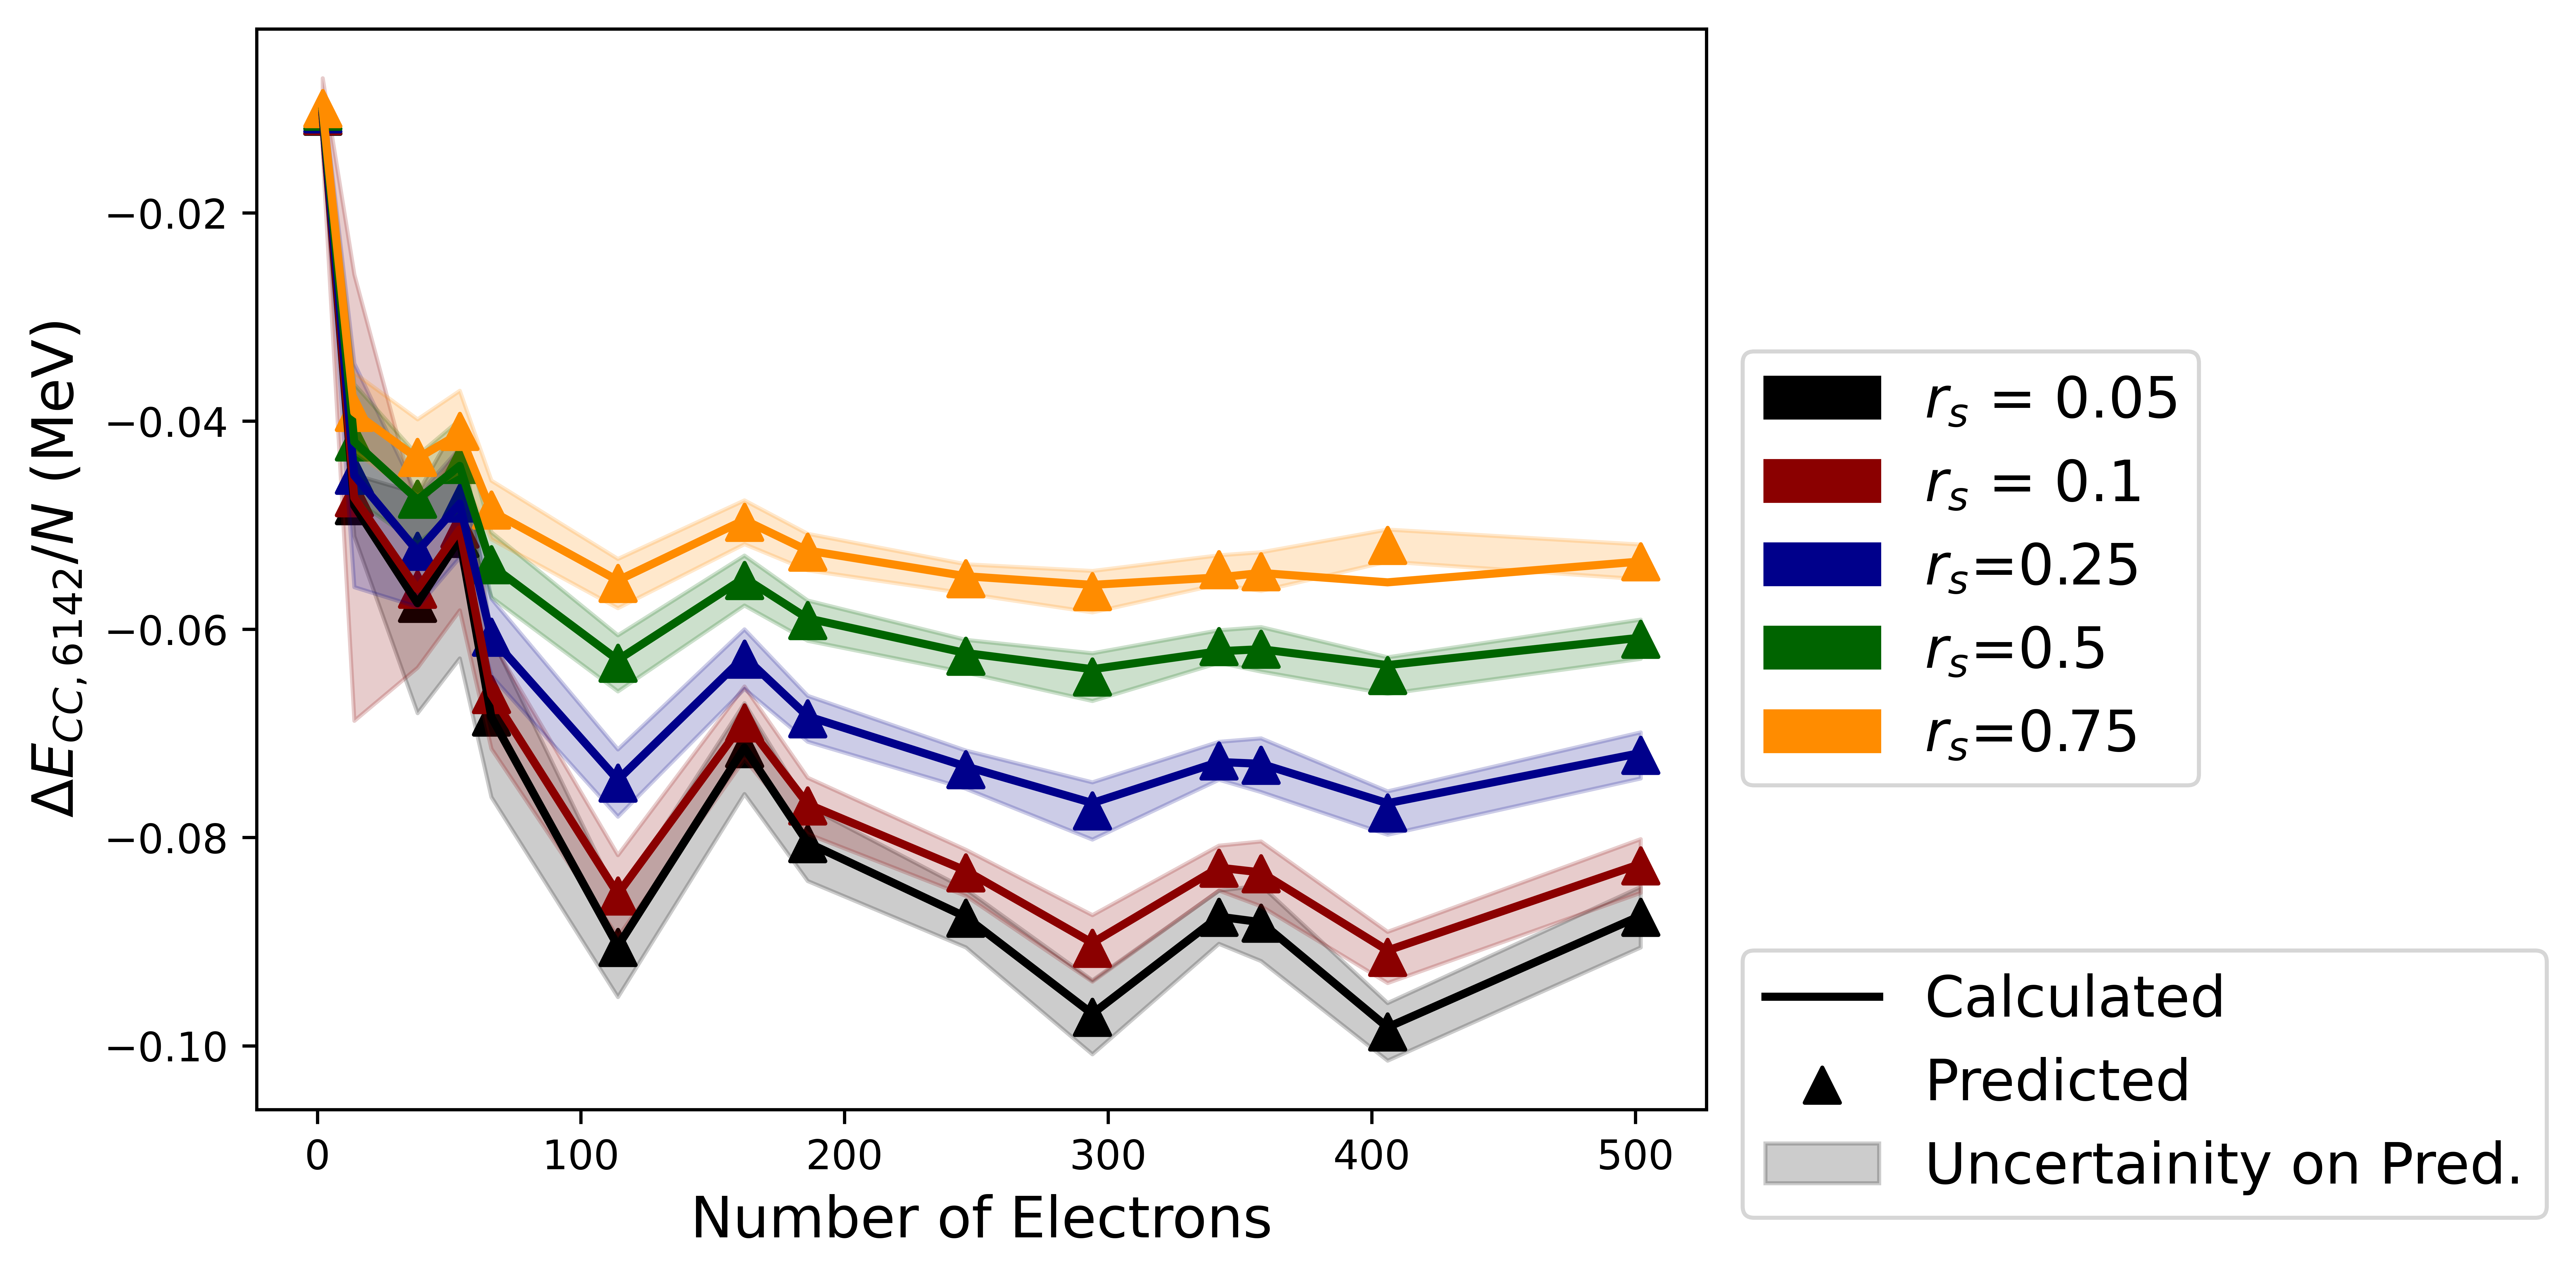
\includegraphics[scale=0.75]{Images/Chapter7/ElectronGas/BRR_EG_MSU_uncertainities.png}
    \captionof{figure}{The results from performing an SRE extrapolation in terms of M for various numbers of electrons and values of r$_s$.  Results are plotted against $\Delta E_{CC,6142}$.}
    \label{brr_eg}
\end{center}


%% ADD SRE TO OTHER EXTRAPOLATIONS
Finally, we can compare the performance of the SRE algorithm to the traditional extrapolation methods we analyzed in Fig. \ref{fig:compare_no_sre}.  For the HEG at $r_s$ = 0.5, if we add the SRE predictions to the others, we get Fig. \ref{fig:compare_sre}.  We can see that the SRE predictions are much closer than any other methods and provide a reasonable approximation to the converged correlation energies, even at high numbers of electrons.

\begin{figure}
    \centering
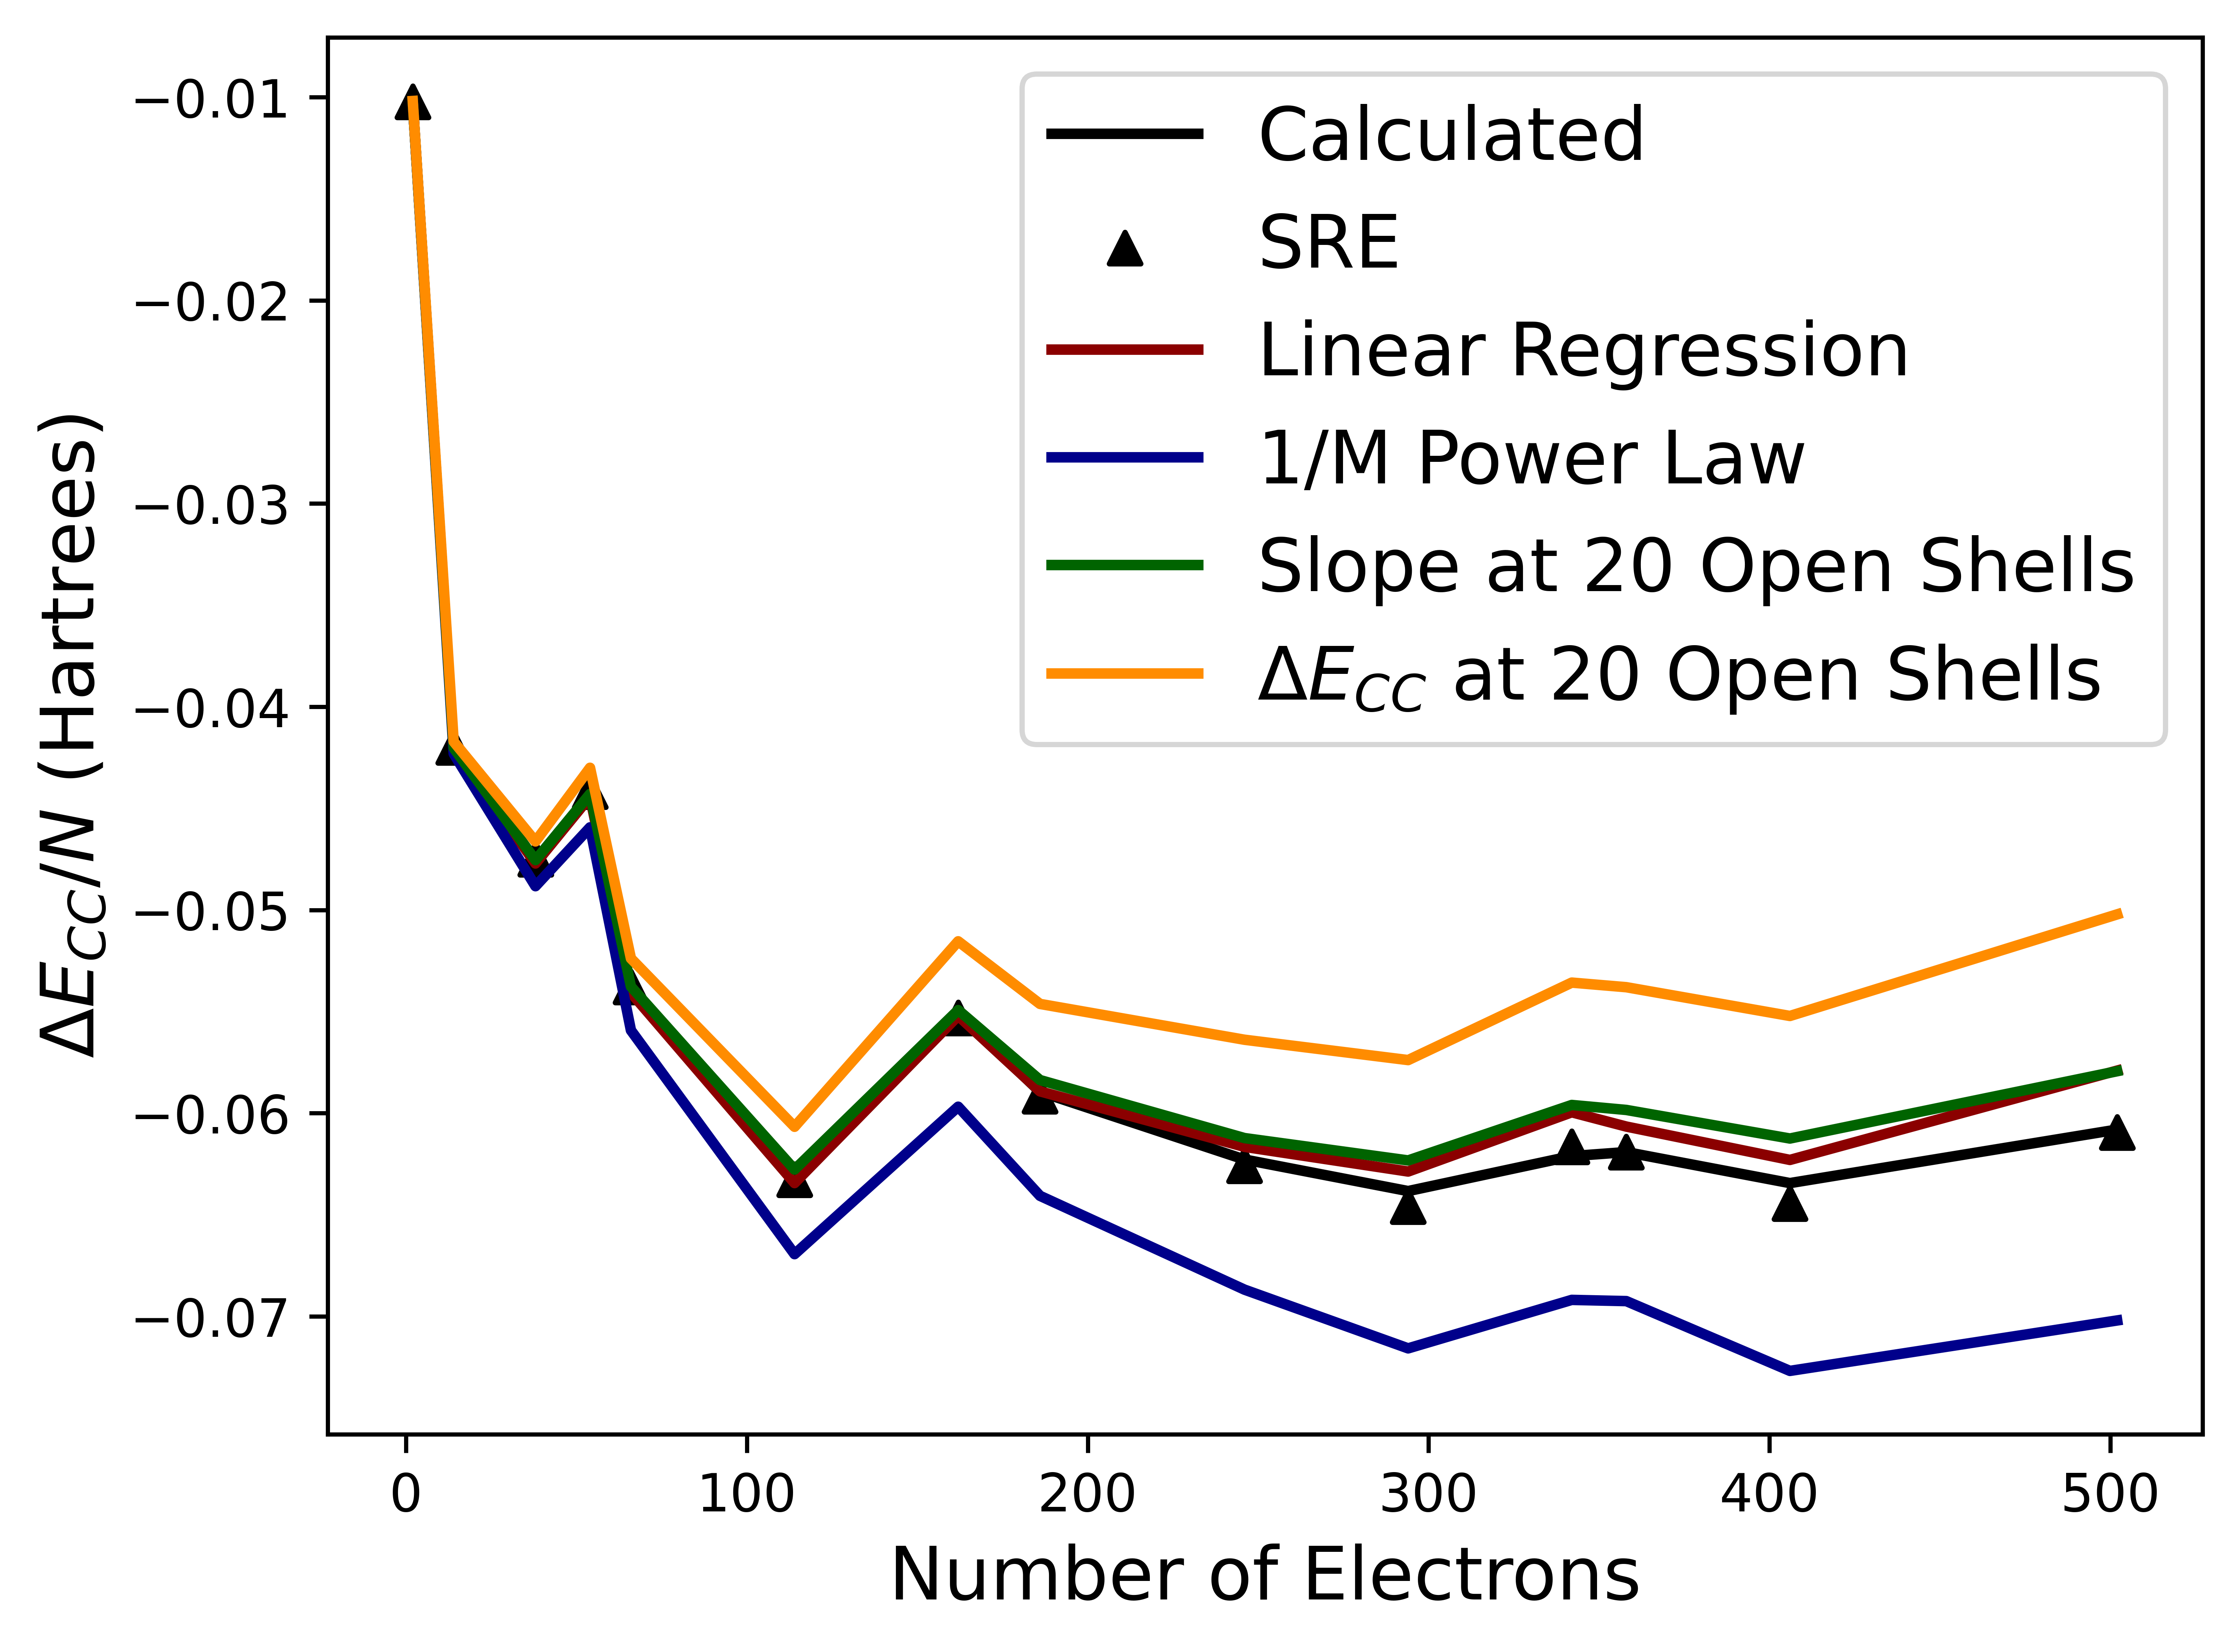
\includegraphics[scale=0.75]{Images/Chapter7/ElectronGas/EG_extrapolation_compare.png}
    \caption{Here, with have recreated Fig. \ref{fig:compare_no_sre}, but have added the SRE results, which have an average percent error of 0.31$\%$.}
    \label{fig:compare_sre}
\end{figure}

%% CONCLUDE
In this section, we have developed the first Bayesian implementation of the SRE method. It has the accuracy of the ridge regression implementation developed in the previous section but without the ambiguity of choosing the algorithm's hyperparameters. Additionally, Bayesian ridge regression provides uncertainties in its predictions, which are helpful in a scientific context. Overall, the SRE method with Bayesian ridge regression is the most promising of the methods attempted so far to remove the basis incompleteness errors.